% ----- APPENDIX D ------------------%
%                                    %
%      Lock Acquisition              %
% ---------------------------------- %
\chapter{Lock Acquisition}
\label{app:LA}

\begin{figure}[!h]
\centerline{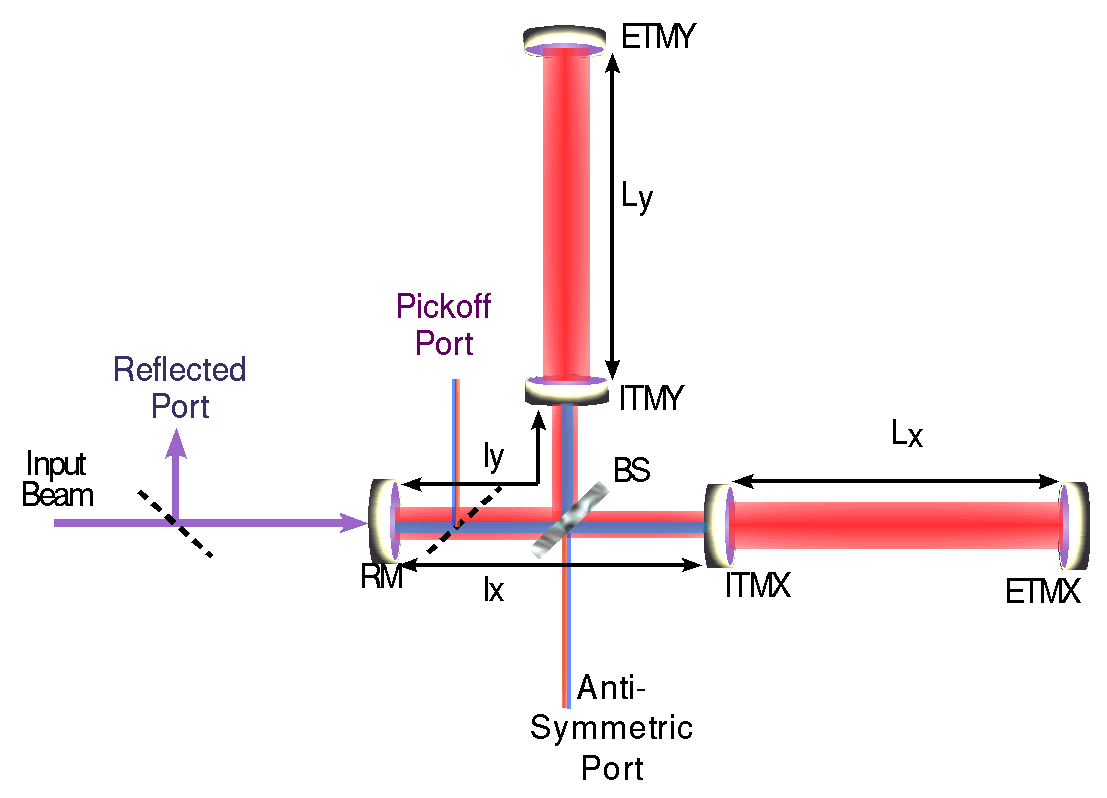
\includegraphics[angle=0,width=6.5in]{Figures/Chap3/IFO2.png}}
\end{figure}

This appendix briefly describes lock acquistion. To acquire lock means
to take the interferometer from an uncontrolled state where the mirrors
swing around and the interferometer 'flashes' through resonances to the
'locked state' where the light is resonant in the interferometer and the
length control loops have been switched on. The lock acquistion scheme is 
described in detail in Matt Evans'  thesis~\cite{Matt:Thesis} and in a 
related paper~\cite{Matt:LApaper}.

In this scheme, various power levels and servo error signals are used to estimate
the field amplitudes for the carrier and sidebands at the 3 signal ports. These
estimates are then used in the real time digital length control system to dynamically
calculate coefficients of an input matrix. This input matrix is what takes the
6 demodulated outputs from the 3 signal ports and produces 4 servo error signals. The
inputs to the matrix calculation (power levels, etc.) are acquired at 16 kHz and so the
matrix is calculated at 16 kHz.

One of the chief difficulties in acquiring lock is the notion of a threshold velocity.
The threshold velocity, $v_t$, is the velocity beyond which the chances of acquiring
lock become small or when the Mean Time To Lock, MTTL, exceeds $\sim$10 minutes.

It is easy to estimate this velocity for a single arm cavity given some of the
optics' and electronics' parameters. In the limit of small velocities, as the
cavity length sweeps through a resonance, there is enough time for the field to
buld up to a steady-state inside. In this limit, the cavity's error signal will
be mostly linear in the region around the resonance and we can define a fringe
width, $x_{\tiny fringe}$, as

\begin{equation}
x_{\mbox{\tiny fringe}} = \frac{\lambda}{2 \, \mathcal{F}}
\end{equation}
which is $\approx3 \times 10^{-9}$ meters for the LIGO arm cavities. Since the distance
is so small we can also approximate the mirror velocity as being constant throughout
the fringe crossing and then say that the crossing time is just, 
$t_c = x_{\mbox{\tiny fringe}}/v_t$, at the threshold velocity.

The other factors which determine the threshold velocity have to do with the 
control system:
\begin{itemize}
\item What is the maximum force that the control system can apply to the mirror?
\item How fast is the control system triggered when the cavity approaches resonance?
\end{itemize}

To lock, the linear momentum of the mirror must be reduced far enough that the
cavity stays resonant long enough for the field to build up. In the case of a single
arm, this condition is trivially met since the cavity time constant is of order 1 ms. 
In the case of the full interferometer, the relevant time constant is that of the coupled 
cavity resonance which is more like 1 second. To a good approximation this means
that the mirror momentum must be reduced to zero. The momentum change effected
by a constant force is $\Delta p = F \, t_c$. Combining this with the expression
for the threshold velocity, we an expression for, $F_{req}$, the required force:

\begin{equation}
F_{req} = \frac{m v}{t_c} = \frac{m v^2}{x_{\mbox{\tiny fringe}}}
\label{eq:LockingForce}
\end{equation}
Equation~\ref{eq:LockingForce} highlights very simply why the interferometers'
duty cycles are so sensitive to seismic noise. Since the threshold velocity
goes like the velocity squared, a slight noise increase can make the average
required force exceed the limits of the electronics and push the interferometer
into the realm where the MTTL = hours. This exceeds the patience of even the
most devoted interferometrist.

As shown in Section~\ref{sec:CoilDriver}, the coil driver for the optic could output
a maximum current of $150 V / 160 \Omega \simeq 1$ Ampere. To protect the actuator coil
from overheating, the amplifier has been limited to a maximum impulsive current 
of 400 mA (and a slow blow fuse to prevent extended operation above 150 mA).
With four coils, each having a force coefficient of 0.016 N/A, we get that the
maximum applicable force is $\sim$25 mN. This gives a threshold velocity of
$\sim$4 microns/second.

The other factor is the delay between the time the cavity approaches resonance
and when the servo turns on and pushes the mirror in the direction which slows
it down. The light level from a single arm cavity resonance is $\approx$1000X
smaller than the level of the light during the full interferometer lock. This
makes the SNR small enough that the trigger threshold for acquisition has been
set to 10-15\% of the single arm level and a digital filter is employed to
reduce the sensitivity to the high frequency electronics noise. The result is 
a delay in the lock acquisition turn on process and an overall increase of the
MTTL.
 

%\begin{itemize}
%\item Does the LA code push the right way all the time?
%\item What is the delay? (smoothing, etc.)
%\end{itemize}





